% !TeX program = xelatex
\documentclass[a4paper,10pt]{article}

% ============================================================================
% ១. កញ្ចប់បណ្ណាល័យ និងការកំណត់ទំព័រ (Packages & Page Setup — តាមគំរូ ls_plan.tex)
% ============================================================================
\usepackage[a4paper, left=0.95cm, right=0.95cm, top=0.85cm, bottom=0.92cm, footskip=0.52cm]{geometry}
\usepackage{amsmath}
\usepackage{unicode-math}
\usepackage{fontspec}
\usepackage{longtable, array, multirow, colortbl}
\usepackage[table]{xcolor}
\usepackage{enumitem}
\usepackage{pifont}
\usepackage{fancyhdr}
\usepackage{tikz}
\usetikzlibrary{calc, arrows.meta, decorations.pathreplacing, patterns, positioning, babel}

\makeatletter
\let\@expl@@@mark@update@singlecol@structures@@\relax
\makeatother

% --- ប្រព័ន្ធស្វែងរកទីតាំងពុម្ពអក្សរស្វ័យប្រវត្តិ (Windows Local + Cloud Repo fonts/) ---
\providecommand{\NGSFindFonts}{%
  \IfFileExists{C:/Windows/Fonts/cambria.ttc}{%
    \def\NGSSysPath{C:/Windows/Fonts/}%
    \def\NGSUserPath{C:/Users/KIT/AppData/Local/Microsoft/Windows/Fonts/}%
  }{%
    \IfFileExists{./fonts/KhmerOSsiemreap.ttf}{\def\NGSSysPath{./fonts/}\def\NGSUserPath{./fonts/}}{%
    \IfFileExists{../fonts/KhmerOSsiemreap.ttf}{\def\NGSSysPath{../fonts/}\def\NGSUserPath{../fonts/}}{%
    \IfFileExists{../../fonts/KhmerOSsiemreap.ttf}{\def\NGSSysPath{../../fonts/}\def\NGSUserPath{../../fonts/}}{%
    \IfFileExists{../../../fonts/KhmerOSsiemreap.ttf}{\def\NGSSysPath{../../../fonts/}\def\NGSUserPath{../../../fonts/}}{%
    \IfFileExists{../../../../fonts/KhmerOSsiemreap.ttf}{\def\NGSSysPath{../../../../fonts/}\def\NGSUserPath{../../../../fonts/}}{%
    \IfFileExists{../../../../../fonts/KhmerOSsiemreap.ttf}{\def\NGSSysPath{../../../../../fonts/}\def\NGSUserPath{../../../../../fonts/}}{%
    \IfFileExists{../../../../../../fonts/KhmerOSsiemreap.ttf}{\def\NGSSysPath{../../../../../../fonts/}\def\NGSUserPath{../../../../../../fonts/}}{%
      \def\NGSSysPath{../../../../../../../fonts/}\def\NGSUserPath{../../../../../../../fonts/}%
    }}}}}}}%
  }%
}
\NGSFindFonts

% ============================================================================
% ២. កំណត់ពុម្ពអក្សរ (Fonts — តាមគំរូ ls_plan.tex)
% ============================================================================
\setmathfont[Path={\NGSSysPath}, FontIndex=1, Scale=1.02]{cambria.ttc}
\defaultfontfeatures{Ligatures=TeX}

\setmainfont[
  Path={\NGSUserPath},
  Extension=.ttf,
  Script=Khmer,
  BoldFont={KhmerOSsiemreap},
  BoldFeatures={FakeBold=1.8},
  ItalicFont={KhmerOSsiemreap},
  ItalicFeatures={FakeSlant=0.25},
  BoldItalicFont={KhmerOSsiemreap},
  BoldItalicFeatures={FakeBold=1.8, FakeSlant=0.25}
]{KhmerOSsiemreap}

\newfontfamily\muol[Path={\NGSUserPath}, Extension=.ttf, Script=Khmer]{KhmerOSmuollight}
\newfontfamily\Tacteing[Path={\NGSUserPath}, Extension=.TTF]{TACTENG}
\newfontfamily\TimesEn[Path={\NGSSysPath}, Extension=.ttf, BoldFont={timesbd}, ItalicFont={timesi}, BoldItalicFont={timesbi}]{times}
\newfontfamily\CalibriFont[Path={\NGSSysPath}, Extension=.ttf]{calibri}
\newfontfamily\CourierCirc[Path={\NGSSysPath}, Extension=.ttf]{cour}

\XeTeXlinebreaklocale "km"
\XeTeXlinebreakskip = 0pt plus 1pt minus 0.1pt

% ============================================================================
% ៣. ពណ៌ និងការតុបតែង (Colors & Styles)
% ============================================================================
\definecolor{stepbg}{HTML}{D9D9D9}
\definecolor{headgray}{HTML}{E6E6E6}
\definecolor{emphred}{HTML}{C00000}

\pagestyle{fancy}
\fancyhf{}
\renewcommand{\headrulewidth}{0pt}
\fancyfoot[R]{\CalibriFont\fontsize{9pt}{11pt}\selectfont\thepage}

\setlength{\parindent}{0pt}
\setlength{\parskip}{0pt}
\setlength{\tabcolsep}{4.5pt}
\setlength{\LTpre}{2pt}
\setlength{\LTpost}{2pt}

\newcolumntype{L}[1]{>{\raggedright\arraybackslash}p{#1}}
\newcolumntype{C}[1]{>{\centering\arraybackslash}p{#1}}

% ============================================================================
% ៤. ពាក្យបញ្ជាជំនួយ (Helper Macros)
% ============================================================================
\newcommand{\en}[1]{{\TimesEn #1}}
\newcommand{\enbf}[1]{{\TimesEn\bfseries #1}}
\newcommand{\khmflourish}{{\Tacteing\fontsize{15pt}{15pt}\selectfont 3}}
\newcommand{\wcirc}{{\CourierCirc\fontsize{9.5pt}{11pt}\selectfont o}}
\newcommand{\ditem}{{\fontsize{7.5pt}{10pt}\selectfont\ding{117}}\ }
\newcommand{\fiveE}[1]{\textcolor{emphred}{\CalibriFont\bfseries #1}}
\newcommand{\redsub}[1]{\textcolor{emphred}{#1}}
\newcommand{\timenote}[1]{\textcolor{emphred}{\textit{#1}}}
\newcommand{\stepheader}[1]{\multicolumn{3}{|c|}{\cellcolor{stepbg}\muol #1} \\ \hline}
\newcommand{\cfig}[1]{{\centering\vspace{3pt}#1\vspace{3pt}\par}}
\newcommand{\cnum}[1]{\mbox{\fontsize{10.5pt}{12pt}\selectfont\ding{\numexpr181+#1\relax}}}
\newcommand{\unit}[1]{\,\text{\en{#1}}}
\newcommand{\riel}{\,\text{៛}}
\newcommand{\graybox}[1]{\colorbox{headgray}{\strut #1}}

% ============================================================================
% ៥. រូបភាព TikZ ស-ខ្មៅ សម្រាប់បង្រៀនលើក្ដារខៀន និងសន្លឹកកិច្ចការ (B&W Diagrams)
% ============================================================================

% ១. E1 Engage: អន្ទាក់បំបាត់តួ -1 ពេលចាប់កត្តារួម 5x(x+2) - (x+2)
\newcommand{\figEngageALGFiveSeven}{%
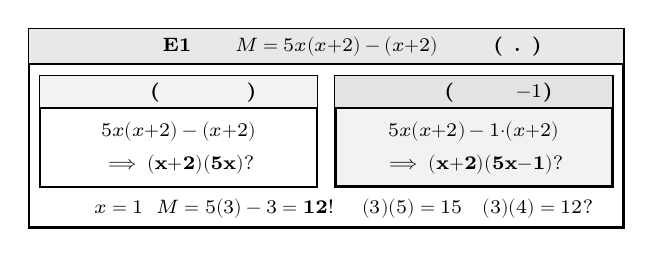
\begin{tikzpicture}[x=1cm, y=1cm, every node/.style={font=\scriptsize, text=black}]
  \draw[black, line width=0.9pt] (0,0) rectangle (7.55,2.52);
  \fill[gray!18] (0,2.08) rectangle (7.55,2.52);
  \draw[black, line width=0.6pt] (0,2.08) -- (7.55,2.08);
  \node at (3.775,2.30) {\textbf{បេសកកម្ម \en{E1}៖ ដាក់ $M = 5x(x{+}2) - (x{+}2)$ ជាកត្តា (ទំ.៦៩)}};

  % Student A
  \draw[black, line width=0.8pt] (0.14,0.52) rectangle (3.66,1.92);
  \fill[gray!10] (0.14,1.52) rectangle (3.66,1.92);
  \draw[black, line width=0.5pt] (0.14,1.52) -- (3.66,1.52);
  \node at (1.90,1.72) {\textbf{សិស្ស ក (បំបាត់តួខាងក្រោយ)}};
  \node at (1.90,1.22) {$5x(x{+}2) - (x{+}2)$};
  \node at (1.90,0.80) {$\implies \mathbf{(x{+}2)(5x)}$?};

  % Student B
  \draw[black, line width=0.95pt, fill=gray!10] (3.89,0.52) rectangle (7.41,1.92);
  \fill[gray!22] (3.89,1.52) rectangle (7.41,1.92);
  \draw[black, line width=0.55pt] (3.89,1.52) -- (7.41,1.52);
  \node at (5.65,1.72) {\textbf{សិស្ស ខ (រក្សាមេគុណ $-1$)}};
  \node at (5.65,1.22) {$5x(x{+}2) - 1{\cdot}(x{+}2)$};
  \node at (5.65,0.80) {$\implies \mathbf{(x{+}2)(5x{-}1)}$?};

  \node at (3.775,0.24) {\textbf{តេស្ត $x = 1$៖} $M = 5(3) - 3 = \mathbf{12}$! តើ $(3)(5)=15$ ឬ $(3)(4)=12$?};
\end{tikzpicture}}

% ២. E2 Explore: កត្តារួមជាកន្សោម (ទំ.៦៩) និងសមភាពសំខាន់ៗបញ្ច្រាស (ទំ.៦៩--៧០)
\newcommand{\figExploreALGFiveSeven}{%
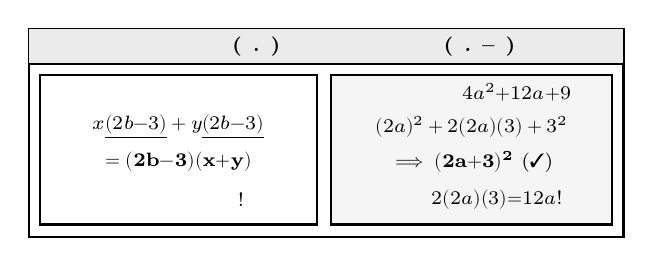
\begin{tikzpicture}[x=1cm, y=1cm, every node/.style={font=\scriptsize, text=black}]
  \draw[black, line width=0.9pt] (0,0) rectangle (7.55,2.64);
  \fill[gray!16] (0,2.20) rectangle (7.55,2.64);
  \draw[black, line width=0.6pt] (0,2.20) -- (7.55,2.20);
  \node at (3.775,2.42) {\textbf{កត្តារួមជាកន្សោម (ទំ.៦៩) និងការផ្ទៀងត្រីធាការេទ្វេធា (ទំ.៦៩--៧០)}};

  % Left: Chunking common binomial factor
  \draw[black, line width=0.8pt] (0.14,0.16) rectangle (3.66,2.06);
  \node at (1.90,1.84) {\textbf{ចាប់កត្តារួមជាកន្សោម}};
  \node at (1.90,1.40) {$x\underline{(2b{-}3)} + y\underline{(2b{-}3)}$};
  \node at (1.90,0.96) {$= \mathbf{(2b{-}3)(x{+}y)}$};
  \node at (1.90,0.48) {គូសបន្ទាត់ក្រោមកត្តារួម!};

  % Right: Perfect square trinomial check
  \draw[black, line width=0.8pt, fill=gray!8] (3.84,0.16) rectangle (7.41,2.06);
  \node at (5.625,1.84) {\textbf{ផ្ទៀងការេទ្វេធា $4a^2{+}12a{+}9$}};
  \node at (5.625,1.40) {$(2a)^2 + 2(2a)(3) + 3^2$};
  \node at (5.625,0.96) {$\implies \mathbf{(2a{+}3)^2}$ (\ding{51})};
  \node at (5.625,0.48) {តួកណ្ដាល $2(2a)(3){=}12a$!};
\end{tikzpicture}}

% ៣. E3 Explain: សង្ខេបរូបមន្តដាក់ជាផលគុណកត្តា (ទំ.៦៨--៧០)
\newcommand{\figRuleALGFiveSeven}{%
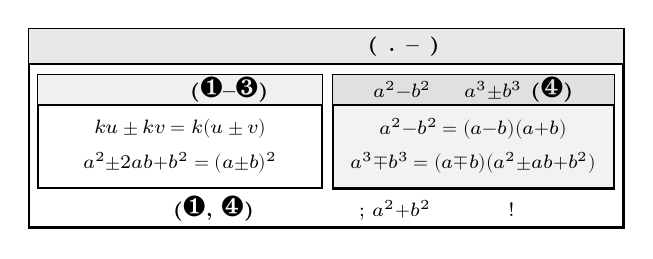
\begin{tikzpicture}[x=1cm, y=1cm, every node/.style={font=\scriptsize, text=black}]
  \draw[black, line width=0.9pt] (0,0) rectangle (7.55,2.52);
  \fill[gray!18] (0,2.08) rectangle (7.55,2.52);
  \draw[black, line width=0.6pt] (0,2.08) -- (7.55,2.08);
  \node at (3.775,2.30) {\textbf{ក្បួនដាក់កន្សោមជាផលគុណកត្តា (ទំ.៦៨--៧០)}};

  % Left: GCF + Square
  \draw[black, line width=0.8pt] (0.12,0.50) rectangle (3.72,1.94);
  \fill[gray!12] (0.12,1.56) rectangle (3.72,1.94);
  \draw[black, line width=0.55pt] (0.12,1.56) -- (3.72,1.56);
  \node at (1.92,1.75) {\textbf{កត្តារួម និងការេ (\cnum{1}--\cnum{3})}};
  \node at (1.92,1.26) {$ku \pm kv = k(u \pm v)$};
  \node at (1.92,0.82) {$a^2{\pm}2ab{+}b^2 = (a{\pm}b)^2$};

  % Right: Diff of squares & cubes
  \draw[black, line width=0.95pt, fill=gray!10] (3.86,0.50) rectangle (7.43,1.94);
  \fill[gray!24] (3.86,1.56) rectangle (7.43,1.94);
  \draw[black, line width=0.6pt] (3.86,1.56) -- (7.43,1.56);
  \node at (5.645,1.75) {\textbf{$a^2{-}b^2$ និង $a^3{\pm}b^3$ (\cnum{4})}};
  \node at (5.645,1.26) {$a^2{-}b^2 = (a{-}b)(a{+}b)$};
  \node at (5.645,0.82) {$a^3{\mp}b^3 = (a{\mp}b)(a^2{\pm}ab{+}b^2)$};

  \node at (3.775,0.24) {\textbf{ចំណាំ (\cnum{1}, \cnum{4})៖} ចាប់កត្តារួមមុនគេ; $a^2{+}b^2$ បំបែកមិនបានទេ!};
\end{tikzpicture}}

% ៤. E4 Elaborate: កត្តារួមបូកសមភាពសំខាន់ៗ (ទំ.៧០, ៧៤)
\newcommand{\figElaborateALGFiveSeven}{%
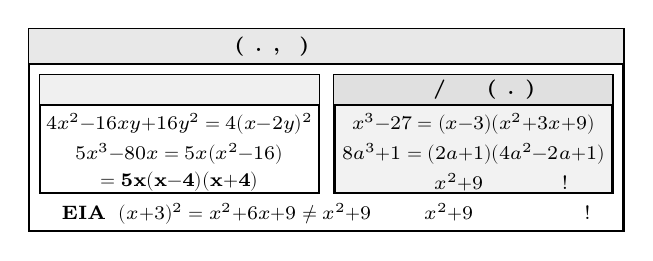
\begin{tikzpicture}[x=1cm, y=1cm, every node/.style={font=\scriptsize, text=black}]
  \draw[black, line width=0.9pt] (0,0) rectangle (7.55,2.56);
  \fill[gray!18] (0,2.12) rectangle (7.55,2.56);
  \draw[black, line width=0.6pt] (0,2.12) -- (7.55,2.12);
  \node at (3.775,2.34) {\textbf{លំហាត់គំរូ (ទំ.៧០, ៧៤)៖ កត្តារួមរួមបញ្ចូលសមភាពសំខាន់ៗ}};

  % Left
  \draw[black, line width=0.8pt] (0.14,0.48) rectangle (3.68,1.98);
  \fill[gray!12] (0.14,1.60) rectangle (3.68,1.98);
  \draw[black, line width=0.55pt] (0.14,1.60) -- (3.68,1.60);
  \node at (1.91,1.79) {\textbf{ចាប់កត្តារួមរួចបំបែកបន្ត}};
  \node at (1.91,1.36) {$4x^2{-}16xy{+}16y^2 = 4(x{-}2y)^2$};
  \node at (1.91,0.98) {$5x^3{-}80x = 5x(x^2{-}16)$};
  \node at (1.91,0.62) {$= \mathbf{5x(x{-}4)(x{+}4)}$};

  % Right
  \draw[black, line width=0.95pt, fill=gray!10] (3.88,0.48) rectangle (7.41,1.98);
  \fill[gray!24] (3.88,1.60) rectangle (7.41,1.98);
  \draw[black, line width=0.6pt] (3.88,1.60) -- (7.41,1.60);
  \node at (5.645,1.79) {\textbf{ផលដក/បូកគូប (ទំ.៧០)}};
  \node at (5.645,1.36) {$x^3{-}27 = (x{-}3)(x^2{+}3x{+}9)$};
  \node at (5.645,0.98) {$8a^3{+}1 = (2a{+}1)(4a^2{-}2a{+}1)$};
  \node at (5.645,0.62) {ប្រយ័ត្ន៖ $x^2{+}9$ បំបែកមិនបានទេ!};

  \node at (3.775,0.22) {\textbf{\en{EIA}៖} $(x{+}3)^2 = x^2{+}6x{+}9 \neq x^2{+}9$ ដូច្នេះ $x^2{+}9$ មិនអាចដាក់ជាកត្តាទេ!};
\end{tikzpicture}}

% ៥. E5 Evaluate: ជម្រើសវិនិច្ឆ័យ A-D ដាក់ 3x^2 - 12 ជាផលគុណកត្តាឱ្យអស់លទ្ធភាព
\newcommand{\figExitALGFiveSeven}{%
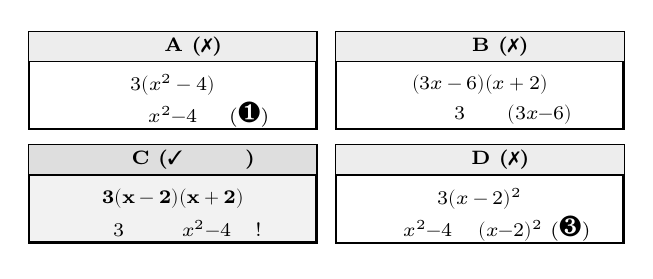
\begin{tikzpicture}[x=1cm, y=1cm, every node/.style={font=\scriptsize, text=black}]
  % Choice A
  \draw[black, line width=0.8pt] (0,1.44) rectangle (3.65,2.68);
  \fill[gray!14] (0,2.30) rectangle (3.65,2.68);
  \draw[black, line width=0.5pt] (0,2.30) -- (3.65,2.30);
  \node at (1.825,2.49) {\textbf{ជម្រើស \en{A} (\ding{55})}};
  \node at (1.825,2.00) {$3(x^2 - 4)$};
  \node at (1.825,1.62) {មិនទាន់បំបែក $x^2{-}4$ អស់ (\cnum{1})};

  % Choice B
  \draw[black, line width=0.8pt] (3.90,1.44) rectangle (7.55,2.68);
  \fill[gray!14] (3.90,2.30) rectangle (7.55,2.68);
  \draw[black, line width=0.5pt] (3.90,2.30) -- (7.55,2.30);
  \node at (5.725,2.49) {\textbf{ជម្រើស \en{B} (\ding{55})}};
  \node at (5.725,2.00) {$(3x - 6)(x + 2)$};
  \node at (5.725,1.62) {សល់កត្តារួម $3$ ក្នុង $(3x{-}6)$};

  % Choice C (Correct)
  \draw[black, line width=1.0pt, fill=gray!10] (0,0) rectangle (3.65,1.24);
  \fill[gray!26] (0,0.86) rectangle (3.65,1.24);
  \draw[black, line width=0.55pt] (0,0.86) -- (3.65,0.86);
  \node at (1.825,1.05) {\textbf{ជម្រើស \en{C} (\ding{51} ត្រឹមត្រូវ)}};
  \node at (1.825,0.56) {$\mathbf{3(x - 2)(x + 2)}$};
  \node at (1.825,0.18) {ចាប់ $3$ រួចបំបែក $x^2{-}4$ អស់!};

  % Choice D
  \draw[black, line width=0.8pt] (3.90,0) rectangle (7.55,1.24);
  \fill[gray!14] (3.90,0.86) rectangle (7.55,1.24);
  \draw[black, line width=0.5pt] (3.90,0.86) -- (7.55,0.86);
  \node at (5.725,1.05) {\textbf{ជម្រើស \en{D} (\ding{55})}};
  \node at (5.725,0.56) {$3(x - 2)^2$};
  \node at (5.725,0.18) {ច្រឡំ $x^2{-}4$ ជា $(x{-}2)^2$ (\cnum{3})};
\end{tikzpicture}}

% ============================================================================
% ៦. ចាប់ផ្ដើមឯកសារ (Document Body)
% ============================================================================
\begin{document}
\fontsize{10pt}{15.2pt}\selectfont

% --- ក្បាលរដ្ឋបាល (Administrative Header) ---
\begin{center}
  {\muol\fontsize{11pt}{16pt}\selectfont ព្រះរាជាណាចក្រកម្ពុជា}\\[2pt]
  {\muol\fontsize{11pt}{16pt}\selectfont ជាតិ សាសនា ព្រះមហាក្សត្រ}\\[-2pt]
  \khmflourish
\end{center}
\vspace{-4pt}

{\muol\fontsize{10pt}{15pt}\selectfont
មន្ទីរអប់រំ យុវជន និងកីឡា ខេត្តកំពង់ធំ\\
ការិយាល័យអប់រំ យុវជន និងកីឡា ស្រុកកំពង់ស្វាយ\\
អនុវិទ្យាល័យព្រះក្រសាំង}

\vspace{2pt}
\begin{center}
  {\muol\fontsize{12pt}{18pt}\selectfont កិច្ចតែងការបង្រៀន}
\end{center}
\vspace{1pt}

% --- ព័ត៌មានទូទៅ (General Metadata) ---
\begin{tabular}{@{}p{1.85cm}p{3.25cm}@{\hspace{4pt}:\hspace{6pt}}p{12.65cm}@{}}
  & - \quad មុខវិជ្ជា          & គណិតវិទ្យា ថ្នាក់ទី៨ (ពីជគណិត) \\
  & - \quad ចំណងជើងមេរៀន & មេរៀនទី៥៖ កន្សោមពីជគណិត \\
  & - \quad ចំណងជើងរង      & ៤.១–៤.២ ការដាក់កន្សោមជាផលគុណកត្តាតាមកត្តារួម និងសមភាពសំខាន់ៗ \\
  & - \quad រយៈពេល             & ១ ម៉ោងសិក្សា (៥០ នាទី) \\
  & - \quad បង្រៀនដោយ         & ហុក ប៊ុនថែន \\
  & - \quad កាលបរិច្ឆេទ        & ថ្ងៃសុក្រ ទី១១ ខែធ្នូ ឆ្នាំ២០២៦ \\
\end{tabular}

\vspace{4pt}

% --- I. វត្ថុបំណង ---
{\muol\enbf{I.} វត្ថុបំណង}\par\vspace{2pt}
\begin{tabular}{@{}p{0.55cm}p{2.55cm}@{\hspace{2pt}:\hspace{6pt}}L{15.4cm}@{}}
  & \wcirc វិជ្ជាសម្បទា   & សិស្សប្រាប់និយមន័យនៃការដាក់កន្សោមជាផលគុណកត្តា និងលំដាប់ជំហានតាមកត្តារួម និងតាមសមភាពសំខាន់ៗ $(a\pm b)^2$, $a^2-b^2$, $a^3\pm b^3$ បានត្រឹមត្រូវ (ទំ.៦៨–៧០) ។ \\[2pt]
  & \wcirc បំណិនសម្បទា & សិស្សដាក់កន្សោមពីជគណិតជាផលគុណកត្តាដោយចាប់កត្តារួម (ឯកធា ឬទ្វេធា) និងដោយប្រើសមភាពសំខាន់ៗលើសន្លឹកកិច្ចការបានត្រឹមត្រូវអស់លទ្ធភាព ។ \\[2pt]
  & \wcirc ចរិយាសម្បទា  & សិស្សមានទម្លាប់ពិនិត្យចាប់កត្តារួមមុនគេ និងផ្ទៀងផ្ទាត់ផលគុណកត្តាទៅនឹងកន្សោមដើមប្រកបដោយភាពម៉ត់ចត់ ។ \\
\end{tabular}

\vspace{3pt}

% --- II. សម្ភារៈឧបទេស (Zero-LCD & Fill-In Worksheet Context) ---
{\muol\enbf{II.} សម្ភារៈឧបទេស}\par\vspace{2pt}
\hspace*{0.55cm}$\bullet$ សៀវភៅសិក្សាគោលថ្នាក់ទី៨ (ទំ.៦៨--៧០, ៧៣--៧៤) ក្ដារខៀន ដីស/ហ្វឺត បន្ទាត់ត្រង់ និង\textbf{សន្លឹកកិច្ចការសិស្សបំពេញចន្លោះ ស-ខ្មៅ} (កូដ \en{ALG57} ទំព័រ ១--២ សម្រាប់សិស្ស និងទំព័រ ៣ ប្លង់ក្ដារខៀន/ចម្លើយគ្រូ — គ្មានប្រើ \en{LCD})

\vspace{3pt}

% --- III. វិធីសាស្រ្តបង្រៀន ---
{\muol\enbf{III.} វិធីសាស្រ្តបង្រៀន}\par\vspace{2pt}
\begin{tabular}{@{}p{0.55cm}p{2.55cm}@{\hspace{2pt}:\hspace{6pt}}L{15.4cm}@{}}
  & $\bullet$ គោលវិធី      & សិស្សមជ្ឈមណ្ឌល (សន្លឹកកិច្ចការបំពេញចន្លោះជាគោល + ការពិភាក្សាជាក្រុមតូច ៣ នាក់) \\
  & $\bullet$ យុទ្ធវិធីបង្រៀន & គំរូស្ថាបនានិយម \en{5Es} រួមបញ្ចូល \textit{ការមើលកន្សោមជាប្លុករួម (\en{Structure Sense / Chunking})} និង \textit{ការវិភាគកំហុសបំបាត់តួ $\pm 1$} \\
\end{tabular}

\vspace{4pt}

% --- IV. ដំណើរការបង្រៀន (50-Minute 5E Flow) ---
{\muol\enbf{IV.} ដំណើរការបង្រៀន}\par\vspace{1pt}

\renewcommand{\arraystretch}{1.15}
\begin{longtable}{|L{5.50cm}|L{7.90cm}|L{4.80cm}|}
\hline
\multicolumn{1}{|c|}{\cellcolor{headgray}\muol សកម្មភាពគ្រូ} &
\multicolumn{1}{c|}{\cellcolor{headgray}\muol ខ្លឹមសារមេរៀន} &
\multicolumn{1}{c|}{\cellcolor{headgray}\muol សកម្មភាពសិស្ស} \\[2pt]
\hline
\endfirsthead

\hline
\multicolumn{1}{|c|}{\cellcolor{headgray}\muol សកម្មភាពគ្រូ} &
\multicolumn{1}{c|}{\cellcolor{headgray}\muol ខ្លឹមសារមេរៀន} &
\multicolumn{1}{c|}{\cellcolor{headgray}\muol សកម្មភាពសិស្ស} \\[2pt]
\hline
\endhead

\hline
\endfoot

% ==================== ជំហានទី១ (2min) ====================
\stepheader{ជំហានទី១ \enbf{(}រដ្ឋបាលថ្នាក់\enbf{)}}
$\bullet$ ពិនិត្យវត្តមាន អនាម័យ និងសណ្ដាប់ធ្នាប់ថ្នាក់រៀន \par
$\bullet$ រៀបចំក្រុមតូច ៣ នាក់ និងចែក\textbf{សន្លឹកកិច្ចការសិស្ស} (\en{ALG57} ទំព័រ ១–២)
&
$\bullet$ រដ្ឋបាលថ្នាក់ អនាម័យ និងវិន័យសិក្សា \par
$\bullet$ ចែកសន្លឹកកិច្ចការម្នាក់ ១ សន្លឹក សម្រាប់បំពេញតាមដំណាក់កាល \en{E1--E5}
&
$\circ$ ប្រធានថ្នាក់រាយការណ៍វត្តមានសិស្ស \par
$\circ$ ទទួលសន្លឹកកិច្ចការ សរសេរឈ្មោះ និងអង្គុយតាមក្រុម ៣ នាក់ \\
\hline

% ==================== ជំហានទី២ (9min: កំណែ ≤3m + រំលឹក 3m + E1 3m) ====================
\stepheader{ជំហានទី២ \enbf{(}កិច្ចការផ្ទះ \enbf{+} ទំនាក់ទំនងមេរៀនថ្មី\enbf{)}}
\ditem \textbf{កំណែកិច្ចការផ្ទះ (\enbf{$\le$ 3 min})} \par
$\bullet$ ហៅសិស្ស ២ នាក់ឡើងកែលំហាត់ទំ.៦៦–៦៧ និងទំ.៧៣ \en{\#10} ឃ, ង លើក្ដារខៀន
&
\hspace*{0.15cm}\redsub{កំណែកិច្ចការផ្ទះ (ទំ.៦៦–៦៧ និង ទំ.៧៣ \en{\#10})} \par
$\bullet$ \textbf{ទំ.៦៦–៦៧៖} $(3x+4y)^3 = 27x^3+108x^2y+144xy^2+64y^3$; \ $(\sqrt{2}a-3b)(2a^2+3\sqrt{2}ab+9b^2) = 2\sqrt{2}a^3-27b^3$ \par
$\bullet$ \textbf{\en{\#10} ឃ, ង៖} ឃ) $-3x^2 - 9xy$; \ ង) $-9x^2 - 9x - 9$
&
$\circ$ ផ្ទៀងចម្លើយ និងកែតម្រូវចូលសៀវភៅកិច្ចការផ្ទះ \\[3pt]

\ditem \textbf{រំលឹកមេរៀនទាក់ទង (\enbf{3min})} \par
$\bullet$ សួរ៖ «បើពន្លាត $3(x+y)$ បាន $3x+3y$ ចុះបើបម្លែងបញ្ច្រាសពី $3x+3y$ វិញបានអ្វី? ចុះ $a^2 - b^2$ ស្មើផលគុណអ្វី?»
&
\hspace*{0.15cm}\redsub{រំលឹកលក្ខណៈបំណែងចែកបញ្ច្រាស និងសមភាពសំខាន់ៗ} \par
$\bullet$ លក្ខណៈបំណែងចែកបញ្ច្រាស៖ $3x + 3y = 3(x + y)$ \par
$\bullet$ សមភាពសំខាន់ៗមើលពីស្ដាំមកឆ្វេង៖ $a^2 - b^2 = (a-b)(a+b)$ និង $a^2 \pm 2ab + b^2 = (a \pm b)^2$
&
$\circ$ ឆ្លើយ៖ «ស្មើ $3(x+y)$ និងស្មើ $(a-b)(a+b)$!» \\[3pt]

\fiveE{E1 - Engage (3min)} \timenote{(កុំទាន់ផ្តល់ចម្លើយ)} \par
\ditem \textbf{បេសកកម្មអន្ទាក់បំបាត់តួ $-1$ (សន្លឹកកិច្ចការ \en{E1})} \par
$\bullet$ ឱ្យសិស្សអានប្រអប់ \en{E1} ហើយតេស្តដោយជំនួស $x = 1$ ដើម្បីជ្រើសរើសរវាងសិស្ស ក និងសិស្ស ខ
&
\redsub{បេសកកម្ម \en{E1}៖ ដាក់ $M = 5x(x+2) - (x+2)$ ជាកត្តា (ទំ.៦៩)} \par
$\bullet$ \textbf{សិស្ស ក} ចាប់ $(x+2)$ បាន $(x+2)(5x)$ (បំបាត់តួក្រោយ)! \par
$\bullet$ \textbf{សិស្ស ខ} ចាប់ $(x+2)$ បាន $(x+2)(5x - 1)$! តើអ្នកណាត្រូវ?
&
$\circ$ ជំនួស $x = 1$ ពិភាក្សាជាគូ និងគូស \ding{51} ក្នុងប្រអប់ \en{E1} \\[3pt]

&
\cfig{\figEngageALGFiveSeven}
& \\
\hline

% ==================== ជំហានទី៣ (17min: E2 11m + E3 6m) ====================
\stepheader{ជំហានទី៣ \enbf{(}ខ្លឹមសារមេរៀនថ្មី\enbf{)}}
\fiveE{E2 - Explore (11min)} \par
$\bullet$ សរសេរចំណងជើងរង \textbf{៤. ការដាក់កន្សោមជាផលគុណកត្តា (៤.១–៤.២)} លើក្ដារខៀន \par
\ditem \textbf{សកម្មភាព ១៖ កត្តារួមជាឯកធា និងទ្វេធា (ទំ.៦៨–៦៩, \enbf{5min}, \en{E2-A})} \par
$\bullet$ ឱ្យសិស្សគូសបន្ទាត់ក្រោមកត្តារួម រួចបំពេញឧទាហរណ៍ទំ.៦៨–៦៩ លើ \en{E2-A}
&
៤.១ ការដាក់ជាផលគុណកត្តាតាមកត្តារួម (ទំ.៦៨–៦៩) \par
$\bullet$ \textbf{កត្តារួមជាឯកធា៖} $3x + 3y + 3z = \mathbf{3(x + y + z)}$; \quad $6a^2b - 9ab^2 = \mathbf{3ab(2a - 3b)}$ \par
$\bullet$ \textbf{កត្តារួមជាកន្សោម (ទំ.៦៩)៖} $x(2b-3) + y(2b-3) = \mathbf{(2b-3)(x+y)}$ \par
\hspace*{0.15cm}លំហាត់គំរូ៖ $(3x+2y)(x+1) - y(x+1) = (x+1)(3x+2y-y) = \mathbf{(x+1)(3x+y)}$
&
$\circ$ គូសបន្ទាត់ក្រោមកត្តារួម និងបំពេញកត្តាលើ \en{E2-A} \\[3pt]

\ditem \textbf{សកម្មភាព ២៖ ប្រើសមភាពសំខាន់ៗ (ទំ.៦៩–៧០, \enbf{6min}, \en{E2-B})} \par
$\bullet$ ឱ្យសិស្សផ្ទៀងទម្រង់ $(a\pm b)^2$, $a^2-b^2$ និង $a^3\pm b^3$ លើ \en{E2-B}
&
៤.២ ប្រើសមភាពសំខាន់ៗ (ទំ.៦៩–៧០) \par
$\bullet$ \textbf{រូបមន្ត $(a\pm b)^2$៖} $4a^2+12a+9 = \mathbf{(2a+3)^2}$; \quad $\dfrac{x^2}{4}-4x+16 = \mathbf{\left(\dfrac{x}{2}-4\right)^2}$; \quad $x^2+10x+25 = \mathbf{(x+5)^2}$ \par
$\bullet$ \textbf{រូបមន្ត $a^2-b^2$ និង $a^3\pm b^3$៖} $a^2-25 = \mathbf{(a-5)(a+5)}$; \quad $8x^3+y^3 = \mathbf{(2x+y)(4x^2-2xy+y^2)}$; \quad $27y^3-64 = \mathbf{(3y-4)(9y^2+12y+16)}$
&
$\circ$ កំណត់ $a, b$ ផ្ទៀងតួកណ្ដាល និងសរសេរផលគុណកត្តាលើ \en{E2-B} \\[3pt]

&
\cfig{\figExploreALGFiveSeven}
& \\[3pt]

% --- E3 Explain (6min) ---
\fiveE{E3 - Explain (6min)} \par
$\bullet$ ដឹកនាំសិស្សសង្ខេបនិយមន័យ និងរូបមន្តបញ្ច្រាសទាំង ៥ (ទំ.៦៨–៧០)
&
$\bullet$ \textbf{និយមន័យ និងរូបមន្តបញ្ច្រាស (ទំ.៦៨–៧០)៖} \par
\hspace*{0.15cm}– កត្តារួម៖ $ku \pm kv = \graybox{$k(u \pm v)$}$; \quad ការេទ្វេធា៖ $a^2 \pm 2ab + b^2 = \graybox{$(a \pm b)^2$}$ \par
\hspace*{0.15cm}– ផលដកការេ៖ $a^2 - b^2 = \graybox{$(a-b)(a+b)$}$; \quad គូប៖ $a^3 \mp b^3 = (a\mp b)(a^2\pm ab+b^2)$
&
$\circ$ បំពេញប្រអប់រូបមន្តបញ្ច្រាសលើ \en{E3} \\[3pt]

$\bullet$ ភ្ជាប់\textbf{ធនាគារហេតុផល \cnum{1}--\cnum{4}} លើក្ដារខៀន និងសន្លឹកកិច្ចការ
&
\textbf{ធនាគារហេតុផល (\en{Warrant Bank})៖} \par
\cnum{1} \textbf{ចាប់កត្តារួមមុនគេជានិច្ច៖} ត្រូវពិនិត្យចាប់កត្តារួមធំបំផុតចេញមុននឹងប្រើសមភាពសំខាន់ៗ \par
\cnum{2} \textbf{មេគុណបង្កប់ $\pm 1$៖} ពេលចាប់តួទាំងមូលចេញជាកត្តារួម ត្រូវរក្សាតួ $\pm 1$ ក្នុងវង់ក្រចក
&
$\circ$ ផ្ទៀងលេខកូដ \cnum{1}--\cnum{2} លើសន្លឹកកិច្ចការ \\[3pt]

&
\cnum{3} \textbf{ផ្ទៀងតួកណ្ដាល $2ab$៖} មុនដាក់ជា $(a\pm b)^2$ ត្រូវផ្ទៀងថាតួកណ្ដាលពិតជាស្មើ $\pm 2ab$
&
$\circ$ ផ្ទៀងលេខកូដ \cnum{3} លើសន្លឹកកិច្ចការ \\[3pt]

&
\cnum{4} \textbf{ហាមបំបែក $a^2 + b^2$៖} ផលបូកពីរការេ $a^2+b^2$ មិនអាចដាក់ជាផលគុណកត្តាក្នុង $\mathbb{R}$ បានទេ
&
$\circ$ ផ្ទៀងលេខកូដ \cnum{4} លើសន្លឹកកិច្ចការ \\[3pt]

&
\cfig{\figRuleALGFiveSeven}
& \\
\hline

% ==================== ជំហានទី៤ (20min: E4 10m + E5 10m) ====================
\stepheader{ជំហានទី៤ \enbf{(}ពង្រីកចំណេះដឹង\enbf{)}}
\fiveE{E4 - Elaborate (10min)} \par
\ditem \textbf{លំហាត់គំរូ៖ កត្តារួមរួមបញ្ចូលសមភាពសំខាន់ៗ (ទំ.៧០, ៧៤)} \par
$\bullet$ ឱ្យសិស្សដោះស្រាយលំហាត់គំរូទំ.៧០ និងទំ.៧៤ \en{\#13} ច លើ \en{E4}
&
\textbf{លំហាត់គំរូពង្រីក (ទំ.៧០ និង ទំ.៧៤)៖} \par
$\bullet$ \textbf{១) ចាប់កត្តារួម និងការេទ្វេធា (ទំ.៧០, ៧៤)៖} \par
\hspace*{0.15cm}-- $4x^2 - 16xy + 16y^2 = 4(x^2 - 4xy + 4y^2) = \graybox{$4(x - 2y)^2$}$ \par
\hspace*{0.15cm}-- $2m^2 + \sqrt{2}mn + \dfrac{n^2}{4} = \left(\sqrt{2}m + \dfrac{n}{2}\right)^2$ \par
\hspace*{0.15cm}-- $5x^3 - 80x = 5x(x^2 - 16) = \graybox{$5x(x - 4)(x + 4)$}$ \par
$\bullet$ \textbf{២) លំហាត់គំរូគូប (ទំ.៧០)៖} \par
\hspace*{0.15cm}-- $x^3 - 27 = \mathbf{(x - 3)(x^2 + 3x + 9)}$; \quad $8a^3 + 1 = \mathbf{(2a + 1)(4a^2 - 2a + 1)}$
&
$\circ$ ចាប់កត្តារួម និងប្រើសមភាពសំខាន់ៗលើ \en{E4} ត្រឹមត្រូវ \\[3pt]

&
\cfig{\figElaborateALGFiveSeven}
& \\[3pt]

$\bullet$ សួរសំណួរឆ្លុះបញ្ចាំង \textbf{\en{EIA Looking-Back}} (\enbf{1min})
&
\textbf{\en{EIA Looking-Back}៖} «ហេតុអ្វី $x^2 + 9$ មិនអាចដាក់ជា $(x+3)(x+3)$ ឬ $(x-3)(x+3)$ បាន?» ($\to$ ព្រោះ $(x+3)^2 = x^2+6x+9$ រីឯ $(x-3)(x+3) = x^2-9 \neq x^2+9$!)
&
$\circ$ ពន្យល់ដោយពន្លាតផ្ទៀងបញ្ច្រាស (\cnum{4}) \\[3pt]

% --- E5 Evaluate (10min) ---
\fiveE{E5 - Evaluate (10min)} \par
\ditem \textbf{ប្រតិបត្តិជាក្រុមតូច ៣ នាក់ (\enbf{4min}, សន្លឹកកិច្ចការ \en{E5})} \par
$\bullet$ ឱ្យសិស្សធ្វើប្រតិបត្តិទំ.៧០ (ក, គ) និងទំ.៧៣–៧៤ (\en{\#11} ឃ, \en{\#13} ឃ)
&
\textbf{លំហាត់ប្រតិបត្តិ (ទំ.៧០ និង ទំ.៧៣–៧៤)៖} \par
$\bullet$ \textbf{១) ទំ.៧០ (ក, គ)៖} $x^2 - 8x + 16 = \mathbf{(x - 4)^2}$; \quad $n^2 - 12n + 36 = \mathbf{(n - 6)^2}$ \par
$\bullet$ \textbf{២) ទំ.៧៣ \en{\#11} ឃ និង ទំ.៧៤ \en{\#13} ឃ៖} \par
\hspace*{0.15cm}$x(4x-8y) + y(x-2y) = 4x(x-2y) + y(x-2y) = \mathbf{(x-2y)(4x+y)}$; \quad $x^2 - 4y^2 = \mathbf{(x-2y)(x+2y)}$
&
$\circ$ ដាក់ជាផលគុណកត្តាជាក្រុមបានត្រឹមត្រូវទាំង ៤ លំហាត់ \\[3pt]

$\bullet$ ឱ្យក្រុមសិស្សផ្ទៀងផ្ទាត់និងបិទ\textbf{បេសកកម្ម \en{E1}} (\enbf{2min})
&
$\bullet$ \textbf{បិទបេសកកម្ម \en{E1}៖} សិស្ស ខ ត្រឹមត្រូវ! $5x(x+2)-(x+2) = \mathbf{(x+2)(5x-1)}$ (ពេល $x=1$: $3\times 4 = 12$ \ding{51})!
&
$\circ$ បិទបេសកកម្ម \en{E1} ឃើញសិស្ស ខ ត្រឹមត្រូវ \\[3pt]

\ditem \textbf{សំណួរវិនិច្ឆ័យ \en{A--D} និងសំបុត្រចេញ (\enbf{4min})} \par
$\bullet$ ឱ្យសិស្សគូសរង្វង់ជម្រើសត្រូវលើសន្លឹកកិច្ចការ រួចលើកម្រាមដៃ ១--៤
&
\centering\textbf{សំណួរវិនិច្ឆ័យ \en{A--D}៖ ដាក់ $3x^2 - 12$ ជាផលគុណកត្តាឱ្យអស់លទ្ធភាព}\par
\textbf{\en{A.}} $3(x^2 - 4)$ \quad
\textbf{\en{B.}} $(3x - 6)(x + 2)$ \quad
\textbf{\en{C.}} $3(x - 2)(x + 2)$ \quad
\textbf{\en{D.}} $3(x - 2)^2$\par
{\itshape (កត់សម្គាល់៖ ត្រូវចាប់កត្តារួម $3$ ចេញមុន រួចបំបែក $x^2 - 4$ បន្ត)}
&
$\circ$ គណនា និងលើកម្រាមដៃ ៣ (\textbf{ជម្រើស \en{C}៖} $3(x - 2)(x + 2)$) \\[3pt]

&
\cfig{\figExitALGFiveSeven}
& \\[3pt]

$\bullet$ បញ្ជាក់ចម្លើយត្រូវ (\textbf{ជម្រើស \en{C}}) និងឱ្យបំពេញសំបុត្រចេញ ៦០ វិនាទី
&
$\bullet$ \textbf{សំបុត្រចេញ (ទំ.៧៤ \en{\#13} ដ)៖} ដាក់ជាផលគុណកត្តា $(x + 1)^2 - 4 = (x+1-2)(x+1+2) = \mathbf{(x - 1)(x + 3)}$ ។
&
$\circ$ បំពេញសំបុត្រចេញលើសន្លឹកកិច្ចការមុនបញ្ចប់ម៉ោង \\
\hline

% ==================== ជំហានទី៥ (≤2min) ====================
\stepheader{ជំហានទី៥ \enbf{(}កិច្ចការផ្ទះ \enbf{+} បណ្ដាំផ្ញើ\enbf{)}}
\timenote{ចំណាយពេលឱ្យតិចបំផុតកុំឱ្យលើស 2min} \par
$\bullet$ ណែនាំប្រអប់កិច្ចការផ្ទះលើសន្លឹកកិច្ចការទំព័រ ២ (ទំ.៧០ និងទំ.៧៣–៧៤)
&
\centering\textbf{កិច្ចការផ្ទះ (សៀវភៅគោល ទំ.៧០ និង ទំ.៧៣–៧៤ \en{\#11, \#12, \#13, \#14})}\par\raggedright
$\bullet$ \textbf{១) ប្រតិបត្តិទំ.៧០ (ខ) និង \en{\#11} ខ (ទំ.៧៣)៖} $y^2 + 10y + 25$ និង $(3a^2 - 12a) - 5(a - 4)$ ។ \par
$\bullet$ \textbf{២) ទំ.៧៤ \en{\#12} ក, ខ; \en{\#13} ក, ង; \en{\#14} ង៖} $(2x-3)(5x-1)-(2x-3)(x+1)$, $(7a-1)^2-(7a-1)(3a+2)$, $a^2-25$, $25x^2-16y^2$ និង $a^2c - 2acx + cx^2$ ។
&
$\circ$ គូសចំណាំកិច្ចការផ្ទះលើសន្លឹកកិច្ចការ \\[3pt]

$\bullet$ ផ្តាំផ្ញើឱ្យអានមុនចំណុច ៤.៣ (របៀបផ្សេងៗក្នុងការដាក់ជាផលគុណកត្តា)
&
$\bullet$ \textbf{បណ្ដាំផ្ញើ៖} អានមុន \textbf{៤.៣ របៀបផ្សេងៗក្នុងការដាក់កន្សោមជាផលគុណកត្តា} (ទំ.៧១–៧២) ។
&
$\circ$ កត់ត្រាបណ្ដាំផ្ញើ ទុកសន្លឹកកិច្ចការក្នុងសៀវភៅ និងជម្រាបលាគ្រូ \\
\hline
\end{longtable}

\vspace{6pt}

% --- ហត្ថលេខា (Signature Block) ---
\begin{flushright}
  \begin{minipage}{8.6cm}
    \centering
    ថ្ងៃសុក្រ ២កើត ខែមិគសិរ ឆ្នាំមមី អដ្ឋស័ក ពុទ្ធសករាជ ២៥៧០\\
    កំពង់ស្វាយ, ថ្ងៃទី១១ ខែធ្នូ ឆ្នាំ២០២៦\\[4pt]
    {\muol គ្រូបង្រៀន}\\[32pt]
    \hfill{\muol ហុក ប៊ុនថែន}\hspace*{1.4cm}
  \end{minipage}
\end{flushright}

\end{document}
